\documentclass[aspectratio=169,11pt]{beamer}

\usepackage[T1]{fontenc}
\usepackage{lmodern}
\usepackage{graphicx}
\usepackage{tikz}
\usetikzlibrary{positioning,arrows.meta}

\definecolor{DeepNavy}{HTML}{13263A}
\definecolor{WarmGold}{HTML}{D9A441}
\definecolor{SoftBlue}{HTML}{EAF1F7}
\definecolor{SoftGold}{HTML}{FFF4D6}
\definecolor{Ink}{HTML}{1E2933}
\definecolor{Muted}{HTML}{5D6B78}
\definecolor{AlertRed}{HTML}{9D2C2C}
\definecolor{Green}{HTML}{2F6F4E}

\setbeamercolor{normal text}{fg=Ink,bg=white}
\setbeamercolor{structure}{fg=DeepNavy}
\setbeamercolor{frametitle}{fg=white,bg=DeepNavy}
\setbeamercolor{title}{fg=white}
\setbeamercolor{subtitle}{fg=SoftBlue}
\setbeamercolor{block title}{fg=white,bg=DeepNavy}
\setbeamercolor{block body}{fg=Ink,bg=SoftBlue}
\setbeamercolor{alertblock title}{fg=white,bg=AlertRed}
\setbeamercolor{alertblock body}{fg=Ink,bg=SoftGold}
\setbeamercolor{exampleblock title}{fg=white,bg=Green}
\setbeamercolor{exampleblock body}{fg=Ink,bg=SoftBlue}
\setbeamercolor{itemize item}{fg=WarmGold}
\setbeamercolor{itemize subitem}{fg=DeepNavy}
\setbeamercolor{enumerate item}{fg=WarmGold}

\setbeamertemplate{navigation symbols}{}
\setbeamertemplate{footline}{%
  \leavevmode%
  \hbox{%
  \begin{beamercolorbox}[wd=.82\paperwidth,ht=2.7ex,dp=1.2ex,leftskip=1em]{author in head/foot}%
    \color{Muted}\small SWOSU Computing Commons \textbullet\ Fun with LaTeX
  \end{beamercolorbox}%
  \begin{beamercolorbox}[wd=.18\paperwidth,ht=2.7ex,dp=1.2ex,rightskip=1em plus1fil]{date in head/foot}%
    \color{Muted}\small \insertframenumber/\inserttotalframenumber
  \end{beamercolorbox}}%
}

\newcommand{\shot}[1]{%
  \begin{center}
  \fbox{\includegraphics[width=0.60\textwidth,height=0.46\textheight,keepaspectratio]{#1}}
  \end{center}
}
\newcommand{\shotsm}[1]{%
  \begin{center}
  \fbox{\includegraphics[width=0.52\textwidth,height=0.40\textheight,keepaspectratio]{#1}}
  \end{center}
}

\title{Fun with LaTeX}
\subtitle{Your First Document That Builds Itself}
\author{SWOSU Computing Commons}
\date{Recitation Toolbox \textbullet\ Documentation and LaTeX}

\begin{document}

{\setbeamercolor{background canvas}{bg=DeepNavy}
\begin{frame}[plain]
  \vspace{1.0cm}
  {\Huge\bfseries\color{white}Fun with LaTeX\par}
  \vspace{0.35cm}
  {\Large\color{SoftBlue}Your First Document That Builds Itself\par}
  \vfill
  {\large\color{WarmGold}The whole idea in one sentence}\par
  \vspace{0.15cm}
  {\Large\color{white}\texttt{hello.tex} is source code. \texttt{hello.pdf} is
  a build artifact. Git tracks the source; one command rebuilds the PDF.\par}
  \vfill
  {\small\color{SoftBlue}Companion slides for the recorded walkthrough --
  see the Fun with LaTeX page on Canvas for the video and the student guide.}
\end{frame}}

\begin{frame}{Source code vs.\ build artifact}
\begin{center}
\resizebox{0.92\textwidth}{!}{%
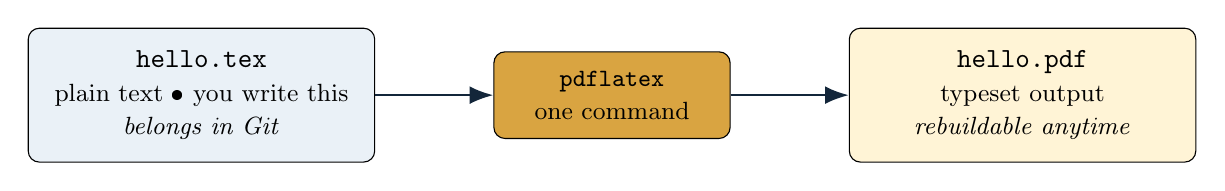
\begin{tikzpicture}[node distance=1.4cm]
  \node[draw,rounded corners,fill=SoftBlue,minimum width=4.4cm,minimum height=1.7cm,align=center] (src)
    {\textbf{\texttt{hello.tex}}\\\small plain text \textbullet\ you write this\\\small \emph{belongs in Git}};
  \node[draw,rounded corners,fill=WarmGold,right=1.5cm of src,minimum width=3.0cm,minimum height=1.1cm,align=center] (mid)
    {\small \texttt{pdflatex}\\\small one command};
  \node[draw,rounded corners,fill=SoftGold,right=1.5cm of mid,minimum width=4.4cm,minimum height=1.7cm,align=center] (pdf)
    {\textbf{\texttt{hello.pdf}}\\\small typeset output\\\small \emph{rebuildable anytime}};
  \draw[-{Latex[length=3mm]},thick,DeepNavy] (src) -- (mid);
  \draw[-{Latex[length=3mm]},thick,DeepNavy] (mid) -- (pdf);
\end{tikzpicture}%
}
\end{center}
\vspace{0.3cm}
\begin{block}{The one question to keep asking}
Which file could I always regenerate, and which one is the thing I actually
authored? Track the source. The artifact is a result.
\end{block}
\end{frame}

\begin{frame}{Predict before you run anything}
\begin{enumerate}
  \item If \texttt{hello.tex} is source and \texttt{hello.pdf} is built from
    it, which file belongs in Git?
  \item \texttt{pdflatex.exe} is on disk. Does the file existing prove the
    tool \emph{works}?
  \item A step deletes four temp files; only two exist. Should it succeed or
    fail?
\end{enumerate}
\vspace{0.4cm}
\begin{alertblock}{Write your answers down}
Every one of these came up as a real snag in the recording. We return to them
at the end.
\end{alertblock}
\end{frame}

\begin{frame}{Open PowerShell -- literally the first step}
\begin{block}{If you have never opened it}
Press the \textbf{Windows key}, type \texttt{powershell}, press
\textbf{Enter}. A dark window with a blinking prompt appears. That prompt is
where every command goes.
\end{block}
\begin{exampleblock}{Get to a working folder}
\texttt{cd \textasciitilde} \\
\texttt{mkdir git -Force ; cd git} \\
\texttt{git clone https://github.com/jeremy-evert/computing\_commons.git} \\
\texttt{cd computing\_commons\textbackslash fun\_with\_LaTeX}
\end{exampleblock}
Run \texttt{Get-Location} and \texttt{ls}. If you see
\texttt{bootstrap\_latex\_project.ps1}, you are in the right place.
\end{frame}

\begin{frame}{Run the bootstrap script once}
\begin{columns}[T]
\begin{column}{0.5\textwidth}
\small
\texttt{.\textbackslash bootstrap\_latex\_project.ps1}
\vspace{0.3cm}

It does six things:
\begin{enumerate}\small
  \item checks the LaTeX toolchain
  \item installs MiKTeX \emph{only if} \texttt{pdflatex} is missing
  \item writes \texttt{hello.tex} (won't overwrite yours)
  \item adds build junk to \texttt{.gitignore}
  \item compiles with \texttt{pdflatex}
  \item writes \texttt{latex\_environment\_report.md}
\end{enumerate}
\end{column}
\begin{column}{0.5\textwidth}
\shot{img/bootstrap_success.png}
\end{column}
\end{columns}
\end{frame}

\begin{frame}{What the toolchain check proves -- and doesn't}
\shotsm{img/bootstrap_success.png}
\begin{block}{Read the table}
\texttt{pdflatex FOUND} means the build can run. The report file it writes --
computer name, tool paths, \texttt{Compiler exit code: 0} -- is your evidence
the PDF built \emph{on your machine}.
\end{block}
\end{frame}

\begin{frame}{The warning that is not a failure}
\begin{alertblock}{You will see this in red-ish text}
\texttt{pdflatex: major issue: So far, no MiKTeX administrator has checked for
updates.}
\end{alertblock}
\begin{block}{It did not stop the build}
The very next lines say \texttt{[SUCCESS] LaTeX is ready and the PDF was
built.} A warning is not a failed build. Open MiKTeX Console and check for
updates when convenient -- then move on.
\end{block}
\end{frame}

\begin{frame}{Open the artifact you just built}
\begin{columns}[c]
\begin{column}{0.46\textwidth}
\shotsm{img/hello_pdf.png}
\end{column}
\begin{column}{0.5\textwidth}
\begin{block}{Verify, don't assume}
One page: title, your name, today's date, three sections, and
\(a^2 + b^2 = c^2\) as real math.
\end{block}
\begin{alertblock}{The habit}
A clean exit code is not proof. Open the PDF and check it is what you meant to
produce.
\end{alertblock}
\end{column}
\end{columns}
\end{frame}

\begin{frame}[fragile]{Edit, rebuild, see the change}
\begin{exampleblock}{The entire skill is this loop}
\begin{verbatim}
code .\hello.tex        # change one true sentence, save

pdflatex -interaction=nonstopmode -halt-on-error \
         -file-line-error hello.tex

Start-Process .\hello.pdf
\end{verbatim}
\end{exampleblock}
Edit source \(\rightarrow\) run one command \(\rightarrow\) inspect the
artifact. Everything else is convenience on top of this.
\end{frame}

\begin{frame}[fragile]{The Makefile detour, snag 1: \texttt{latexmk} needs Perl}
\begin{alertblock}{\texttt{latexmk.exe} was on disk, so it looked usable}
\begin{verbatim}
MiKTeX could not find the script engine 'perl'
which is required to execute 'latexmk'.
\end{verbatim}
\end{alertblock}
\begin{block}{Prediction \#2, answered}
Finding an executable does not prove its dependencies are satisfied.
\texttt{pdflatex} alone already builds this document -- so call it directly and
depend on nothing else.
\end{block}
\end{frame}

\begin{frame}[fragile]{The Makefile detour, snag 2: cleanup that fails on nothing}
\begin{alertblock}{Deleting temp files that were already gone}
\begin{verbatim}
make: *** [Makefile:32: clean] Error 1
\end{verbatim}
The cleanup command returned non-zero because some files did not exist.
\texttt{make} correctly called that a failed step -- and \texttt{rebuild}
depended on \texttt{clean}, so \texttt{pdflatex} never ran.
\end{alertblock}
\begin{block}{Prediction \#3, answered}
``Delete these if they exist'' should \emph{succeed} when they are already
gone.
\end{block}
\end{frame}

\begin{frame}[fragile]{The fix was subtraction}
\begin{exampleblock}{The working \texttt{Makefile} -- four functional lines}
\begin{verbatim}
.PHONY: all
all:
	pdflatex -interaction=nonstopmode -halt-on-error \
	         -file-line-error hello.tex
	powershell.exe -NoProfile -Command \
	  "Start-Process (Resolve-Path 'hello.pdf')"
\end{verbatim}
\end{exampleblock}
No \texttt{latexmk}, no Perl, no cleanup target, no dependency graph. Recipe
lines start with a real \textbf{tab}.
\begin{block}{The rule}
Start with the command that works. Automate \emph{that}. Add complexity only
when the project proves it needs it.
\end{block}
\end{frame}

\begin{frame}{Keep the receipt (Git)}
\shotsm{img/git_receipt.png}
\begin{block}{Commit the history, snags and all}
\texttt{status} \(\rightarrow\) \texttt{add} \(\rightarrow\) \texttt{diff
--cached} \(\rightarrow\) \texttt{commit} \(\rightarrow\) \texttt{pull
--rebase} \(\rightarrow\) \texttt{push}. The history records both the failed
abstraction and the simpler repair -- not something to hide.
\end{block}
\end{frame}

\begin{frame}{The finish line}
\begin{exampleblock}{You are done when you can say}
I turned a text file into a PDF on my own machine with one command. I have the
environment report as evidence it built here. I know which file is source and
which is the artifact, and both are under Git. I hit a build failure, read the
real error, removed what did not earn its place, and got to a working
\texttt{make}.
\end{exampleblock}
\shotsm{img/shipped.png}
\end{frame}

\begin{frame}{Where to go from here}
\begin{itemize}
  \item Full walkthrough video and the step-by-step student guide: the
    \textbf{Fun with LaTeX} page in Computing Commons on Canvas.
  \item Stuck? The student guide has an ``If something goes wrong'' table with
    the exact snags from this recording.
  \item Next: change the document -- add a section, a table, a figure -- then
    \texttt{make} again and watch the artifact follow your source.
\end{itemize}
\vspace{0.4cm}
\begin{block}{The station question}
\emph{Can another human understand and inspect what I did?} A tracked
\texttt{.tex} source plus a rebuildable \texttt{.pdf} is one honest answer.
\end{block}
\end{frame}

\end{document}
